%%%%%%%% FlowSNE theory paper -- ICML 2026 template %%%%%%%%%%%%%%%%%
% Working draft. Numbers in Section 5 come from
% experiments/theory/gauge_checks.py (results/gauge_checks_*.json);
% numbers in Section 6 from the FlowSNE experiment reports cited there.

\documentclass{article}

\usepackage{microtype}
\usepackage{graphicx}
\usepackage{subcaption}
\usepackage{booktabs}
\usepackage{hyperref}
\newcommand{\theHalgorithm}{\arabic{algorithm}}

% blind submission; switch to [preprint] or [accepted] as needed
\usepackage{icml2026}

\usepackage{amsmath}
\usepackage{amssymb}
\usepackage{mathtools}
\usepackage{amsthm}
\usepackage[capitalize,noabbrev]{cleveref}

\theoremstyle{plain}
\newtheorem{theorem}{Theorem}[section]
\newtheorem{proposition}[theorem]{Proposition}
\newtheorem{lemma}[theorem]{Lemma}
\newtheorem{corollary}[theorem]{Corollary}
\theoremstyle{definition}
\newtheorem{definition}[theorem]{Definition}
\newtheorem{assumption}[theorem]{Assumption}
\theoremstyle{remark}
\newtheorem{remark}[theorem]{Remark}

\usepackage[textsize=tiny]{todonotes}

% ---------------------------------------------------------------- macros
\newcommand{\R}{\mathbb{R}}
\newcommand{\T}{\mathbb{T}}
\newcommand{\eps}{\varepsilon}
\newcommand{\1}{\mathbf{1}}
\newcommand{\diag}{\operatorname{diag}}
\newcommand{\Sep}{\mathcal{S}}
\newcommand{\Asym}{\mathcal{A}}
\newcommand{\Grad}{\mathcal{G}}
\newcommand{\Cyc}{\mathcal{C}}
\newcommand{\cyc}{\operatorname{cyc}}
\newcommand{\dv}{\operatorname{div}}
\newcommand{\Ptrue}{P}
\newcommand{\Sk}{\operatorname{Sk}}
\newcommand{\RS}{\operatorname{RS}}
\newcommand{\Leray}{\Pi}
\newcommand{\E}{\mathbb{E}}

\icmltitlerunning{What a Balanced Affinity Sees}

\begin{document}

\twocolumn[
  \icmltitle{What a Balanced Affinity Sees:\\
    Sinkhorn Normalisation as a Helmholtz Projection of Directed Costs}

  \begin{icmlauthorlist}
    \icmlauthor{Nicolas Courty}{ubs}
  \end{icmlauthorlist}
  \icmlaffiliation{ubs}{TODO affiliation}
  \icmlcorrespondingauthor{Nicolas Courty}{TODO}
  \icmlkeywords{neighbour embedding, optimal transport, Sinkhorn, Finsler, Randers, Hodge decomposition, RNA velocity}
  \vskip 0.3in
]

\printAffiliationsAndNotice{}

\begin{abstract}
  Many datasets come with a direction at each point: RNA velocity, a gradient
  field, the velocity of a generative model. A natural way to let a neighbour
  embedding use it is to replace the symmetric ground cost by a
  direction-dependent one, such as a Randers metric, and keep the usual
  entropic affinity. We ask which part of the direction survives the
  normalisation of that affinity. For finite samples, we show that a
  Sinkhorn-balanced affinity is determined by the cost modulo separable
  functions. Its asymmetry therefore carries exactly the cyclic, non-gradient
  part of the cost's asymmetry, and a gradient drift, including a uniform
  one, is pure gauge. In the continuum limit, the Markov chain of a balanced
  affinity transports mass along a field that is divergence-free with
  respect to the sampling density. For the Laplace--Randers kernel this
  field has a closed form: at small drift it is the density-weighted Helmholtz
  projection of the drift onto its solenoidal part, whereas row-stochastic and
  diffusion-map normalisations transport along the whole drift. Two
  ingredients of practical affinities break the gauge. Per-row bandwidth
  calibration leaks gradient drifts at first order, and strongly; a squared
  cost leaks them at third order in the limit, though at first order with a
  small constant at the sample sizes we can simulate. Numerical experiments
  confirm the other predictions quantitatively, and Hodge
  decompositions of real RNA-velocity fields show when balancing helps and
  when it discards the signal.
\end{abstract}

% ======================================================================
\section{Introduction}
\label{sec:intro}

Neighbour embeddings such as SNE, t-SNE and UMAP
\citep{hinton2002sne,vandermaaten2008tsne,mcinnes2018umap} build an affinity
matrix from a symmetric ground cost and fit a low-dimensional layout whose
own affinities match it. Doubly stochastic affinities, computed by
Sinkhorn iterations \citep{sinkhorn1967concerning,cuturi2013sinkhorn},
make every point send and receive the same mass. SNEkhorn
\citep{vanassel2023snekhorn} showed that such marginals, in a symmetric
entropic affinity, fix the hub and density problems of row-normalised
affinities.

Many datasets, however, come with a \emph{direction} at each point: RNA
velocity in single-cell transcriptomics
\citep{lamanno2018rna,bergen2020generalizing}, the gradient of a loss with
respect to activations, the velocity field of a flow-matching model, the
displacement of an optimal-transport plan. A symmetric cost cannot express
``cheaper to move with the flow than against it''. The natural fix is a
Finsler cost, and the simplest Finsler cost is the Randers metric
\citep{randers1941asymmetrical,bao2000introduction}:
\begin{equation}
  F_x(v) = \|v\| + \omega(x)^\top v, \qquad \|\omega\| < 1 .
  \label{eq:randers}
\end{equation}
Plugging such a cost into an entropic affinity is straightforward. It is
much less clear what the resulting affinity actually encodes. The
normalisation step rescales rows and columns, and rescaling can absorb part
of the asymmetry. Indeed, in our experiments a Sinkhorn-balanced Randers
affinity was nearly blind to some drifts and sensitive to others of the same
magnitude.

This paper characterises that behaviour exactly. Our answer is a Helmholtz
decomposition: \emph{a balanced affinity sees the circulation of a drift and
not its gradient part.}

\paragraph{Contributions.}
\begin{itemize}
  \item \textbf{Finite samples (\cref{sec:finite}).} A balanced coupling
    identifies its cost exactly modulo separable functions $f_i+g_j$
    (\cref{thm:identifiability}). Consequently, the cyclic part of
    $\log(P_{ij}/P_{ji})$ equals $-2/\eps$ times the cyclic part of the
    cost's antisymmetric part, for any diagonal-scaling normalisation. What
    differs between normalisations is only how gradient drifts reach the
    marginals, and balancing removes them. A uniform drift is invisible.
    Independently of the cost, the net mass flow of a balanced affinity is
    a pure circulation: it makes no net progress along any potential
    (\cref{prop:netflow}).
  \item \textbf{Continuum limit (\cref{sec:continuum}).} Under a standard
    small-noise ansatz for the Sinkhorn potentials, the transport field of
    a balanced affinity is divergence-free with respect to the sampling
    density $p$ and solves a strictly convex variational problem
    (\cref{thm:continuum}). For the Laplace--Randers kernel it has a closed
    form; at small drift it is $-(d{+}1)\,\Leray_p\,\omega$, the
    $p$-weighted Leray projection. Row-stochastic and diffusion-map
    normalisations instead transport along the centroid field of the Randers
    unit ball \citep{debaussart2026finslerian}, which contains the whole
    drift.
  \item \textbf{Leakage (\cref{sec:leak}).} Practical affinities use a
    squared cost and per-row bandwidths. Per-row bandwidths leak gradient
    drifts at first order, through the part of $\nabla\phi/\sigma$ that is
    not a gradient. In the limit, the squared cost leaks them only at third
    order in their magnitude.
  \item \textbf{Evidence (\cref{sec:exp,sec:real}).} Each prediction is
    checked numerically, and Hodge decompositions of real velocity fields
    explain when a balanced affinity helps (cell-cycle circulation) and
    when it discards most of the signal (developmental trajectories).
\end{itemize}

% ======================================================================
\section{Setting}
\label{sec:setting}

\paragraph{Affinities are diagonal scalings of a kernel.}
Given points $x_1,\dots,x_n$ and a cost matrix $C\in\R^{n\times n}$, not
necessarily symmetric, write $K=\exp(-C/\eps)$ entrywise. The three
normalisations we consider all rescale the rows and the columns of $K$,
\begin{equation}
  \log P_{ij}=-C_{ij}/\eps+\log\alpha_i+\log\beta_j ,
  \label{eq:scaling}
\end{equation}
that is $P=\diag(\alpha)K\diag(\beta)$,
and differ only in how $\alpha,\beta>0$ are chosen.
\begin{itemize}
  \item \emph{Row-stochastic} ($\RS$), as in SNE's conditional affinities:
    $\beta=\1$ and $\alpha_i=1/\big(n\,(K\1)_i\big)$. Each row is a
    softmax of $-C_{i\cdot}/\eps$ and $P\1=\1/n$.
  \item \emph{Diffusion map} with exponent $\theta\in[0,1]$
    \citep{coifman2006diffusion}: with degrees $d=K\1$, first
    $K\leftarrow\diag(d)^{-\theta}K\diag(d)^{-\theta}$, then row
    normalisation. The row factor $d_i^{-\theta}$ cancels, leaving
    $\beta_j=d_j^{-\theta}$ and $\alpha_i=1/\big(n\,(K\beta)_i\big)$:
    a column factor fixed by the degrees, not by a prescribed marginal.
  \item \emph{Balanced} ($\Sk$): $\alpha=u$ and $\beta=v$ are the
    positive vectors, unique up to $(u,v)\mapsto(cu,v/c)$, with
    $u\odot Kv=a$ and $v\odot K^\top u=b$ for prescribed marginals $a,b$
    of equal mass, found by Sinkhorn iterations, here with $a=b=\1/n$.
\end{itemize}
SNE and t-SNE also calibrate a per-row bandwidth $\eps_i$ to a target
perplexity \citep{vladymyrov2013entropic}. That divides row $i$ of $C$ by
$\eps_i$, which is not of the form \eqref{eq:scaling}; we treat it
separately in \cref{sec:leak}.
SNEkhorn \citep{vanassel2023snekhorn} is \emph{not} $\Sk$. It minimises
$\langle P,C\rangle$ under unit row sums, a per-row entropy floor and the
constraint $P=P^\top$, with solution
$P_{ij}=\exp\big((\mu_i+\mu_j-2C_{ij})/(\gamma_i+\gamma_j)\big)$. For
symmetric $P$, $\langle P,C\rangle=\langle P,\tfrac12(C+C^\top)\rangle$, so
SNEkhorn sees only the symmetric part of a cost and discards every drift,
cyclic or not. $\Sk$ drops the symmetry constraint and keeps two free
scalings $u\neq v$. For a symmetric $C$ and equal $\gamma_i$ the two
coincide.

\paragraph{Randers costs.}
A Randers norm \citep{randers1941asymmetrical,bao2000introduction} adds a
linear drift term to the Euclidean norm, $F_x(v)=\|v\|+\omega(x)^\top v$.
It is positive and convex in $v$ if and only if $\|\omega(x)\|<1$, and it
is asymmetric: moving along $\omega$ costs $1+\|\omega\|$ per unit
length, moving against it $1-\|\omega\|$. A correctly fitted $\omega$
thus points \emph{away} from the direction the affinity favours. The
Randers distance $d_F(x\to y)$ is the infimum of
$\int_0^1F_{\gamma(t)}(\dot\gamma)\,dt$ over paths from $x$ to $y$.
It has no closed form when $\omega$ varies, for three reasons
(\cref{app:randers}). In low dimension, $d_F(x_0\to\cdot)$ solves an
eikonal equation, which fast-marching schemes for asymmetric metrics
handle on a grid \citep{sethian2003ordered,mirebeau2014efficient}, one
source at a time. In the $10$ to $50$ dimensions of single-cell data a
grid is out of reach, and graph shortest paths \citep{tenenbaum2000global}
need exponentially many points to converge. Above all, $\omega$ is
measured only at the samples, so the infimum over paths through empty
regions depends on an extension of $\omega$ the data do not support.
We therefore use costs built from the endpoint values
$\omega_i=\omega(x_i)$ only, with $\Delta_{ij}=x_j-x_i$:
\begin{itemize}
  \item \emph{frozen,}
    $\hat d(x_i\to x_j)=\|\Delta_{ij}\|+\omega_i^\top\Delta_{ij}$;
  \item \emph{averaged,}
    $\bar d(x_i\to x_j)=\|\Delta_{ij}\|+\tfrac12(\omega_i+\omega_j)^\top\Delta_{ij}$.
\end{itemize}
Both approximate the cost of the straight segment by a quadrature rule,
left-endpoint and trapezoid, with errors $O(\|\nabla\omega\|r^2)$ and
$O(\|\nabla^2\omega\|r^3)$ at $r=\|\Delta_{ij}\|$. Bending the segment
gains only $O(\|\nabla\omega-\nabla\omega^\top\|^2r^3)$
(\cref{app:randers}). A kernel at bandwidth $\eps$ only weighs pairs with
$r=O(\eps)$, so these errors are small where the affinity looks.
The two closed forms have the \emph{same antisymmetric part}
$\tfrac12(\omega_i+\omega_j)^\top\Delta_{ij}$. They differ only in their
symmetric part, by $\tfrac12(\omega_i-\omega_j)^\top\Delta_{ij}$.

One case is exact. For a \emph{gradient drift} $\omega=\nabla\phi$, the
drift term integrates to $\phi(y)-\phi(x)$ along any path, so straight
lines are geodesics and $d_F(x\to y)=\|y-x\|+\phi(y)-\phi(x)$. No
convexity of $\phi$ is needed. Admissibility only asks $\|\nabla\phi\|<1$,
which makes $\phi$ $1$-Lipschitz and $d_F$ positive off the diagonal.
Convexity would only order the costs: it puts the frozen cost below the
exact one, since $\nabla\phi(x_i)^\top\Delta_{ij}\le\phi_j-\phi_i$.
The averaged form's drift term is then a trapezoid rule for
$\phi_j-\phi_i$, with error $O(\|\nabla^3\phi\|\,r^3)$.

\paragraph{The gauge: separable matrices.}
By \eqref{eq:scaling}, every normalisation adds to $-C/\eps$ a matrix of
the form $f_i+g_j$. Let
\[
  \Sep=\{(f_i+g_j)_{ij}:f,g\in\R^n\}.
\]
If two costs differ by an element of $\Sep$, their kernels differ by
diagonal factors on the left and right. A normalisation that chooses
both scalings itself, such as $\Sk$, absorbs those factors and returns the
same $P$. So $\Sep$ is the set of cost changes that balancing cannot see,
a gauge group in the physicist's sense. \Cref{thm:identifiability} shows that
it is the \emph{only} such set. To read it in terms of drifts, we need to
know which asymmetric costs lie in $\Sep$.

\begin{lemma}[Structure of $\Sep$]
  \label{lem:sep}
  Let $\Asym$ be the antisymmetric $n\times n$ matrices and
  $\Grad=\{(\psi_j-\psi_i)_{ij}:\psi\in\R^n\}\subset\Asym$. Then
  \begin{equation}
    \Sep=\{(s_i+s_j)_{ij}:s\in\R^n\}\oplus\Grad,\qquad \Sep\cap\Asym=\Grad .
    \label{eq:sep}
  \end{equation}
  with $\oplus$ a direct sum of subspaces.
\end{lemma}

\begin{proof}
  Write $f_i+g_j=(s_i+s_j)+(\psi_j-\psi_i)$ with $s=\tfrac12(f+g)$ and
  $\psi=\tfrac12(g-f)$. The first term is symmetric and the second
  antisymmetric, so the sum is direct. If $f_i+g_j$ is antisymmetric, its
  diagonal gives $g=-f$, hence $f_i+g_j=f_i-f_j\in\Grad$.
\end{proof}

The symmetric half, $s_i+s_j$, is a per-point offset, such as a cost of
leaving and entering each point; it carries no direction. The
antisymmetric half is exactly the gradient flows. So among asymmetric
costs, those balancing cannot see are precisely the differences of a
potential, $\psi_j-\psi_i$, and nothing else. A uniform drift
$\omega\equiv c$ is one: $c^\top\Delta_{ij}=\psi_j-\psi_i$ with
$\psi=c^\top x$.

\paragraph{Hodge decomposition: what balancing keeps.}
Write $C=S+A$ with $S$ symmetric and $A_{ij}=\tfrac12(C_{ij}-C_{ji})$, the
extra cost of going $i\to j$ rather than $j\to i$, an edge flow on the
complete graph \citep{jiang2011statistical,lim2020hodge}. By \cref{lem:sep} and
\cref{thm:identifiability}, balancing cannot distinguish $A$ from any
$A+G$, $G\in\Grad$: it sees only the \emph{class} $A+\Grad$. We need a canonical split of $A$
into the part that is lost and the part that is kept. Given symmetric positive edge weights $W$, the
weighted cyclic part of $B\in\Asym$ is
\begin{equation}
  \cyc_W(B) = B-\operatorname*{arg\,min}_{G\in\Grad}\textstyle\sum_{ij}W_{ij}(B_{ij}-G_{ij})^2 .
  \label{eq:cyc}
\end{equation}
Adding $G\in\Grad$ to $B$ shifts the minimiser by $G$, so
$\cyc_W(B+G)=\cyc_W(B)$. Conversely, equal cyclic parts force $B-B'$ to be
a difference of minimisers, a gradient. Hence
$\cyc_W(B)=\cyc_W(B')\iff B-B'\in\Grad$: the cyclic part is a complete
invariant of what balancing sees, for every $W$, and $W$ only chooses the
representative. The normal equations of \eqref{eq:cyc}
give $\sum_jW_{ij}\cyc_W(B)_{ij}=0$ for every $i$: $\cyc_W(B)$ is the
unique element of $B+\Grad$ with no net $W$-flow out of any point.

\begin{itemize}
  \item A \emph{gradient} flow $\psi_j-\psi_i$ is an asymmetry fully
    explained by a scalar ranking, such as a pseudotime. Moving up costs
    more because the target is higher. Its sum around every closed loop
    telescopes to zero.
  \item The \emph{cyclic} part is what no ranking explains. Loop sums
    $B_{i_1i_2}+B_{i_2i_3}+\dots+B_{i_mi_1}$ are unchanged by adding a
    gradient, so they are the observables of the class, and $\cyc_W(B)$
    is the divergence-free flow that carries them. For a Randers drift
    term, the loop sum around a small triangle is $\oint\omega\cdot dx$,
    about the curl of $\omega$ times the area by Stokes' theorem. The
    cyclic part is thus a discrete curl: rotation around the cell cycle,
    or around any loop of states.
\end{itemize}
This is the discrete counterpart of the Helmholtz decomposition
$\omega=\nabla\phi+\omega_{\mathrm{sol}}$; in the continuum limit $W$
becomes the kernel weight times the density, and $\cyc_W$ becomes a
density-weighted Leray projection (\cref{sec:continuum}). On the
$k$-nearest-neighbour graphs used on data, the cyclic part splits further into a local
curl around triangles and a harmonic flow around holes of the graph
\citep{jiang2011statistical}; the cell cycle is such a hole.

% ======================================================================
\section{Finite samples: balanced affinities are gauge invariant}
\label{sec:finite}

\begin{theorem}[Identifiability modulo separable costs]
  \label{thm:identifiability}
  Fix positive marginals $a,b$ with equal mass and $\eps>0$. For a cost $C$,
  let $\Sk(C)$ denote the unique coupling of the form
  $\diag(u)e^{-C/\eps}\diag(v)$ with marginals $a,b$. Then
  \[
    \Sk(C)=\Sk(C') \iff C-C'\in\Sep .
  \]
  In particular, writing $C=S+A$ with $S$ symmetric and $A$ antisymmetric,
  $\Sk(S+A)=\Sk(S+A')$ if and only if $A-A'\in\Grad$.
\end{theorem}

\begin{proof}
  The kernel is entrywise positive, so the scaling exists and the coupling
  is unique \citep{sinkhorn1967concerning}. If $C'_{ij}=C_{ij}+f_i+g_j$, then
  $e^{-C'/\eps}=\diag(e^{-f/\eps})e^{-C/\eps}\diag(e^{-g/\eps})$. The
  diagonal factors are absorbed into $u,v$, so uniqueness gives the same
  coupling. Conversely, if both couplings equal $P$, then
  $\log P_{ij}=\log u_i+\log v_j-C_{ij}/\eps=\log u'_i+\log v'_j-C'_{ij}/\eps$.
  Hence $C-C'\in\Sep$. The second statement follows from \cref{lem:sep}.
\end{proof}

The second statement says that, among all asymmetric information, a
balanced affinity retains exactly the cost's antisymmetric part modulo
gradients. The asymmetry of the coupling itself makes this explicit.

\paragraph{An optimal transport reading.}
$\Sk(C)$ is the entropic optimal transport plan between $a$ and $b$ for
the ground cost $C$ \citep{cuturi2013sinkhorn,peyre2019computational};
with $a=b$ it is an entropic self-transport. The gauge $\Sep$ is then a
familiar freedom of OT. On couplings $P\in\Pi(a,b)$,
$\sum_{ij}P_{ij}(C_{ij}+f_i+g_j)=\langle P,C\rangle+\langle a,f\rangle+\langle b,g\rangle$,
so a separable change shifts every transport cost by the same constant
and leaves the optimal plans unchanged, with or without entropy
\citep{villani2009optimal,santambrogio2015optimal}. Combined with the
classical fact that adding a closed one-form to a Randers metric does not
change its geodesics \citep{bao2000introduction}, this gives the
continuous statement. For an exact drift $\omega=\nabla\phi$ the Randers
cost is $\|y-x\|+\phi(y)-\phi(x)$, so unregularised OT under this cost
between any $\mu$ and $\nu$ has the optimal plans of the Euclidean
$W_1$ problem, and its value is $W_1(\mu,\nu)+\int\phi\,d(\nu-\mu)$. For
self-transport the value is unchanged too. We have not found this stated,
but it follows directly from the two facts above. Three points are
specific to our setting.
\begin{itemize}
  \item \emph{The converse needs entropy.} Optimality of an unregularised
    plan is characterised by $c$-cyclical monotonicity, which involves the
    cost only through alternating cycle sums, and many costs share the
    same optimal plan. An entropic plan determines $\log P$, hence $C$ up
    to $\Sep$ (\cref{thm:identifiability}). This is what makes the cyclic
    part $\cyc_W(A)$ the exact content of a balanced affinity.
  \item \emph{The invariance is tied to the linear cost.} The squared
    Randers cost $(\|\Delta_{ij}\|+\phi_j-\phi_i)^2$ contains the cross
    term $2\|\Delta_{ij}\|(\phi_j-\phi_i)$, which is not separable. This is
    the source of the squared cost's leak in \cref{sec:leak}.
  \item \emph{The normalisations are OT problems with different marginal
    constraints.} $\RS$ is entropic OT with only the row marginal imposed,
    a semi-relaxed problem. Leaving the column marginal free is what lets
    the gradient part through (see below). Unbalanced OT, with
    KL-penalised marginals \citep{chizat2018scaling}, would sit between
    $\RS$ and $\Sk$ and should see the gradient part with a strength set
    by the penalty. We leave this to future work.
\end{itemize}

\begin{corollary}[Cyclic content of any diagonal normalisation]
  \label{cor:cyclic}
  Let $P=\diag(\alpha)e^{-C/\eps}\diag(\beta)$ with $\alpha,\beta>0$. This
  covers row-stochastic, diffusion-map and balanced affinities. Then
  \[
    \log\frac{P_{ij}}{P_{ji}}=-\frac{2}{\eps}A_{ij}+(\chi_j-\chi_i),
    \qquad \chi=\log\beta-\log\alpha ,
  \]
  and therefore $\cyc_W\!\big(\log P-\log P^\top\big)=-\tfrac{2}{\eps}\cyc_W(A)$
  for every weight matrix $W$.
\end{corollary}

The cyclic part of the asymmetry is thus fixed by the cost alone, and is
the same for every normalisation. The normalisations differ in the gradient
part $\chi$, which is set by the marginals, and in what the marginals
themselves are.

\begin{corollary}[Gradient drifts are pure gauge]
  \label{cor:gauge}
  Let $\omega=\nabla\phi$ with $\|\nabla\phi\|<1$. Take the exact Randers
  cost $C_{ij}=\|x_j-x_i\|+\phi(x_j)-\phi(x_i)$ and a single global $\eps$.
  Then $\Sk(C)=\Sk(D)$, where $D_{ij}=\|x_j-x_i\|$, for every choice of
  marginals.
  \begin{itemize}
    \item A \emph{uniform} drift $\omega\equiv c$ is the gradient of
      $c^\top x$, so a balanced affinity cannot detect it at all.
    \item Under the averaged closed form, the cyclic part of the drift term
      is $O(\|\nabla^3\phi\|\,r^3)$ on pairs at distance $r$. It vanishes
      for quadratic $\phi$.
  \end{itemize}
\end{corollary}

\Cref{thm:identifiability} concerns log-ratios. A second, even simpler
fact concerns the mass that actually moves, and it holds for \emph{every}
cost.

\begin{proposition}[Balanced net flow is a circulation]
  \label{prop:netflow}
  Let $P$ have equal marginals, $P\1=P^\top\1=a$. Then the net flow
  $N=P-P^\top$ is divergence-free at every point, $N\1=0$. Equivalently,
  $N\perp\Grad$, and for every $f\in\R^n$
  \[
    \textstyle\sum_{ij}P_{ij}\,(f_j-f_i)=0 .
  \]
  The same holds for every power of the chain $\diag(a)^{-1}P$.
\end{proposition}

\begin{proof}
  $\sum_{ij}P_{ij}(f_j-f_i)=\sum_ja_jf_j-\sum_ia_if_i=0$. Taking
  $f=\1_k$ gives $(N\1)_k=0$. For gradient flows,
  $\langle N,(\psi_j-\psi_i)\rangle=\sum_{ij}N_{ij}(\psi_j-\psi_i)=-2\sum_i\psi_i(N\1)_i=0$.
  The chain $\diag(a)^{-1}P$ has stationary law $a$, and so do its powers.
\end{proof}

So a balanced affinity makes \emph{no net progress along any potential},
for instance along a pseudotime, in any number of steps. It can only
circulate. Progress around a cycle is still possible, because a phase
increment is not the difference of a single-valued function. On a
trajectory with no return path, any local forward motion must be
compensated elsewhere, by mass sent backwards. In this language,
\cref{cor:gauge} says that for a gradient drift the circulation is exactly
that of the symmetric affinity, and \cref{sec:leak} says how much spurious
circulation practical affinities add.

For row-stochastic affinities the same gradient drift is \emph{not}
invisible. With $C=D+G$ and $G_{ij}=\phi_j-\phi_i$,
\[
  \RS(C)_{ij}\propto e^{-D_{ij}/\eps}\,e^{-\phi_j/\eps}.
\]
This is the symmetric affinity with targets reweighted towards low $\phi$,
which is the direction of $-\omega$. The log-asymmetry is still a pure
gradient (\cref{cor:cyclic}), so the information sits entirely in the
column marginal, i.e.\ in where mass is sent. Balancing prescribes that
marginal and so removes the drift. \Cref{sec:continuum} turns this into a
statement about transport.

\begin{remark}[Two readings of a drift]
  Write a drift as a gradient part plus a circulating part. The gradient
  part says \emph{where mass should go}; a normalisation that leaves column
  sums free records it as a marginal tilt. The circulating part says
  \emph{how mass moves at fixed marginals}, and every diagonal
  normalisation records it identically. This is the dual of the snapshot
  non-identifiability of \citet{weinreb2018fundamental}: population
  snapshots constrain the potential part of a dynamics and not its
  rotation, whereas a balanced velocity affinity keeps the rotation and
  discards the potential.
\end{remark}

% ======================================================================
\section{Continuum limit: the balanced transport field}
\label{sec:continuum}

\Cref{cor:cyclic} describes log-ratios, but an embedding uses the affinity
as a Markov chain: the mass $P_{ij}$ that $x_i$ sends to $x_j$. We now
compute where that chain moves mass, as the bandwidth vanishes.

\paragraph{Setting.}
Let $p\in C^2(\T^d)$ be a density on the flat torus with $p\ge p_{\min}>0$.
Let $\omega\in C^2(\T^d;\R^d)$ with $\sup\|\omega\|<1$, and let
$\sigma\in C^2(\T^d)$ be a positive relative bandwidth. The torus avoids
boundaries and curvature terms; see the remark after \cref{cor:laplace} for the harmonic part
it introduces. Let $g:[0,\infty)\to(0,\infty)$ be a decreasing profile.
The two cases of interest are $g(t)=e^{-t}$ (linear cost) and
$g(t)=e^{-t^2/2}$ (squared cost). With $\Delta=y-x$ the torus displacement,
the frozen Randers kernel is
\begin{equation}
  k_h(x,y)=g\!\left(\frac{F_x(\Delta)}{h\,\sigma(x)}\right),
  \qquad F_x(v)=\|v\|+\omega(x)^\top v .
  \label{eq:kernel}
\end{equation}
\begin{itemize}
  \item The \emph{balanced chain} is
    $T_h(x,dy)=u_h(x)\,k_h(x,y)\,v_h(y)\,p(y)\,dy$, with $u_h,v_h$ chosen so
    that $T_h(x,\cdot)$ is a probability and $p$ is stationary:
    $\int p(x)T_h(x,dy)\,dx=p(y)\,dy$. This is the static Schr\"odinger
    problem with both marginals equal to $p$ \citep{leonard2014survey}.
  \item The \emph{row-stochastic chain} is
    $T^{\RS}_h(x,dy)\propto k_h(x,y)\,p(y)\,dy$.
\end{itemize}
The \emph{transport field}, in units of the bandwidth, is
$b_h(x)=h^{-1}\!\int(y-x)\,T_h(x,dy)$.

\paragraph{Tilted log-partition.}
For $\omega\in\R^d$ with $\|\omega\|<1$, define on its open convex domain
\begin{equation}
  \Lambda(\omega,\zeta)=\log\!\int_{\R^d} g\big(F_\omega(v)\big)\,e^{\zeta^\top v}\,dv,
  \qquad M=\nabla_\zeta\Lambda .
  \label{eq:Lambda}
\end{equation}
$M(\omega,\zeta)$ is the mean of the profile tilted by $e^{\zeta^\top v}$.
$\Lambda(\omega,\cdot)$ is a log-Laplace transform of a non-degenerate
measure, hence strictly convex.

\begin{assumption}[Small-noise potentials]
  \label{ass:wkb}
  $\log v_h=\Psi/h+R_h$, with $\Psi\in C^2(\T^d)$, and $R_h$ bounded in
  $C^1$ uniformly in $h$. Moreover $\sigma\nabla\Psi(x)$ lies in the domain
  of $\Lambda(\omega(x),\cdot)$ for every $x$.
\end{assumption}

This is the usual WKB behaviour of Schr\"odinger potentials
\citep{leonard2014survey}. It holds exactly for gradient drifts with the
linear profile: there $v_h=e^{\phi/h}$ times the symmetric scaling.

\begin{theorem}[Balanced transport is $p$-solenoidal; formal]
  \label{thm:continuum}
  Under \cref{ass:wkb}, $b_h\to b$ uniformly, where
  \begin{equation}
    b(x)=\sigma(x)\,M\big(\omega(x),\,\sigma(x)\nabla\Psi(x)\big),
    \qquad \dv(p\,b)=0 .
    \label{eq:b}
  \end{equation}
  The potential $\Psi$ is, up to a constant, the unique minimiser of the
  strictly convex functional
  \begin{equation}
    J(\Psi)=\int_{\T^d}p(x)\,\Lambda\big(\omega(x),\sigma(x)\nabla\Psi(x)\big)\,dx .
    \label{eq:J}
  \end{equation}
  For the row-stochastic chain, by contrast,
  $b^{\RS}_h\to\sigma\,M(\omega,0)=\sigma\,\kappa_g\,c_F$. Here $c_F(x)$ is
  the centroid of the Randers unit ball $\{F_x\le1\}$, and
  $\kappa_g=\int t^{d+1}|g'|\,dt\,/\int t^d|g'|\,dt$.
\end{theorem}

The proof sketch, in three steps (local profile, stationarity,
variational form), is in \cref{app:continuum}.

\Cref{thm:continuum} is the Sinkhorn counterpart of the antisymmetric
limits of \citet{perraultjoncas2011directed} and
\citet{debaussart2026finslerian}. Their row- and $\theta$-normalised
operators converge to transport along the centroid field. Balancing adds
the tilt $\sigma\nabla\Psi$, chosen to cancel exactly the part of that
transport which would change the density.

\subsection{The Laplace--Randers kernel in closed form}

For $g(t)=e^{-t}$ the tilted log-partition is explicit. With
$\eta=\omega-\zeta$,
\begin{equation}
  \Lambda(\omega,\zeta)=\log c_d-\tfrac{d+1}{2}\log\!\big(1-\|\eta\|^2\big),
  \qquad \|\eta\|<1 .
  \label{eq:laplace}
\end{equation}
This follows from $\int e^{-\|v\|-\eta^\top v}dv=c_d(1-\|\eta\|^2)^{-(d+1)/2}$,
which can be checked by integrating in polar coordinates. The Randers unit
ball is an ellipsoid with centroid $c_F=-\omega/(1-\|\omega\|^2)$, and
$\kappa_g=d+1$.

\begin{corollary}[Laplace--Randers, global bandwidth]
  \label{cor:laplace}
  Let $g(t)=e^{-t}$ and $\sigma\equiv1$. Then
  \begin{align*}
    b&=-(d+1)\,\frac{\omega-\nabla\Psi}{1-\|\omega-\nabla\Psi\|^2},\\
    \Psi&\in\operatorname*{arg\,min}_{\Psi}\;-\!\int p\,\log\!\big(1-\|\omega-\nabla\Psi\|^2\big),
  \end{align*}
  whereas $b^{\RS}=-(d+1)\,\omega/(1-\|\omega\|^2)$. Moreover:
  \begin{enumerate}
    \item $b\equiv0$ if and only if $\omega$ is a gradient on $\T^d$.
      This is the continuum version of \cref{cor:gauge}, valid for every
      density $p$.
    \item At small drift, $b=-(d+1)\,\Leray_p\,\omega+O(\|\omega\|^3)$.
      Here $\omega=\nabla\Psi_0+\Leray_p\omega$ is the $p$-weighted
      Helmholtz decomposition, with $\dv(p\,\Leray_p\omega)=0$.
  \end{enumerate}
\end{corollary}

The proof is in \cref{app:continuum}.

So a balanced Laplace--Randers affinity is, to first order, a
\emph{density-weighted Leray projector}: it moves mass along the
$p$-solenoidal part of $-\omega$, and only that. The row-stochastic chain
moves mass along all of $-\omega$. Note that the weight is the sampling
density. Whether a drift counts as circulating depends on how the points
are distributed, not only on the geometry.

On $\T^d$, constant fields are not gradients of periodic functions, so
$\Leray_p$ also keeps a harmonic component; on $\R^d$ with a confining
density, a constant field is the gradient of $c^\top x$ and is invisible,
as in \cref{cor:gauge}.

% ======================================================================
\section{Leakage: what practical affinities let through}
\label{sec:leak}

Neighbour embeddings rarely use a linear cost with one global bandwidth.
SNE-type affinities use a \emph{squared} cost and \emph{per-row}
bandwidths calibrated to a perplexity. Both break the gauge.

\paragraph{Finite samples.}
Both effects multiply the gradient flow $G$ entrywise by a symmetric weight
$m$. If the effective log-kernel has antisymmetric part $-(m\odot G)$, then
for any constant $c$ we have $\cyc_W(m\odot G)=\cyc_W((m-c)\odot G)$, since
$cG\in\Grad$. Therefore
\begin{equation}
  \big\|\cyc_W(m\odot G)\big\|_W\;\le\;\inf_{c}\big\|(m-c)\odot G\big\|_W .
  \label{eq:leakbound}
\end{equation}
The leaked asymmetry is controlled by the \emph{heterogeneity} of $m$ over
the edges that carry weight. The two cases are:
\begin{itemize}
  \item \emph{Squared cost.} With $(D+G)^2=D^2+G^2+2D\odot G$, the weight is
    $m=2D/\eps$, the distance itself. The leak is set by the spread of
    neighbour distances, which shrinks as $1/\sqrt{2d}$ for Gaussian
    neighbourhoods in intrinsic dimension $d$.
  \item \emph{Per-row bandwidths.} Write $\beta_i=1/\eps_i$. The
    antisymmetric part of $\beta_iC_{ij}$ is
    $\tfrac12(\beta_i-\beta_j)S_{ij}+\tfrac12(\beta_i+\beta_j)A_{ij}$. The
    first term is the familiar drift-free asymmetry of SNE conditionals.
    The drift enters with weight $m_{ij}=\tfrac12(\beta_i+\beta_j)$, so it
    leaks in proportion to how much bandwidths vary across edges.
\end{itemize}
In both cases the leak in $\log(P_{ij}/P_{ji})$ is of first order in the
drift. The continuum limit separates the two effects sharply.

\begin{corollary}[Leakage orders]
  \label{cor:leak}
  Under \cref{ass:wkb}, let $\omega=\nabla\phi$ with $\|\nabla\phi\|=O(\rho)$.
  \begin{enumerate}
    \item \textbf{Squared cost, global bandwidth} ($g=e^{-t^2/2}$,
      $\sigma\equiv1$). Then $b=O(\rho^3)$, and $b$ is generically
      non-zero.
    \item \textbf{Linear cost, per-row bandwidth} ($g=e^{-t}$). Then
      $b=-(d+1)\,\sigma^2\,\Leray_{p\sigma^2}(\nabla\phi/\sigma)+O(\rho^3)$.
      This is first order in $\rho$, and it vanishes iff
      $\nabla\phi/\sigma$ is a gradient, i.e.\ iff
      $d\sigma\wedge d\phi=0$.
  \end{enumerate}
\end{corollary}

\begin{proof}[Proof sketch]
  (1) The map $M$ is odd: $M(-\omega,-\zeta)=-M(\omega,\zeta)$.
  Linearising around $0$ for the standard Gaussian profile gives
  $M(\omega,\zeta)=\zeta-s_0\,\omega+O(3)$, with
  $s_0=2\,\E\|v\|^3/d$ and $v\sim\mathcal{N}(0,I_d)$. The linear part of
  the drift is therefore the gauge $\zeta=s_0\nabla\phi$, which is a
  gradient. What remains is the $p$-solenoidal part of a cubic remainder.
  (2) Here $\Lambda$ depends on $\omega-\zeta$ only. So
  $b=\sigma M(\omega,\sigma\nabla\Psi)\approx-(d+1)\,\sigma^2(\omega/\sigma-\nabla\Psi)$.
  Stationarity $\dv(p\,b)=0$ is then the weighted Helmholtz problem with
  weight $p\sigma^2$.
\end{proof}

Perplexity calibration makes $\sigma$ scale roughly like $p^{-1/d}$.
Under per-row bandwidths, a gradient drift is thus invisible only when the
density is constant on the level sets of its potential. This is the
dominant leak at small drift. In the limit, the squared cost leaks less in
transport even though it leaks comparably in log-ratios: what it adds is an
odd, skewed asymmetry whose mean displacement cancels at first order. At
finite sample sizes this cancellation is incomplete (\cref{sec:exp}).

% ======================================================================
\section{Numerical verification}
\label{sec:exp}

We check each statement on synthetic data where the Helmholtz parts of the
drift are known exactly. \Cref{app:protocol} gives the protocol. All
couplings are computed in float64 and balanced to $10^{-11}$.

\paragraph{Finite-sample identities.}
On $400$ points in $\R^5$ with a generic cost:
\begin{itemize}
  \item adding a gradient flow $G$ to the cost changes the balanced
    coupling by $2\times10^{-14}$ in relative $\ell_1$ norm, and the
    row-stochastic one by $0.11$ (\cref{thm:identifiability});
  \item the cyclic part of $\log(P/P^\top)$ equals $-\tfrac2\eps\cyc(A)$ to
    a relative error of $5\times10^{-15}$, although the log-ratio also has
    a large gradient part, $31\%$ of its norm (\cref{cor:cyclic}).
\end{itemize}

\paragraph{Transport fields.}
On the flat torus $\T^2$ with a non-uniform density, we use a drift
$\omega=\rho(\nabla\phi+w)$ whose $p$-weighted decomposition is known by
construction: $\dv(p\,w)=0$. \Cref{fig:fields} shows the result for the
linear Randers cost with a global bandwidth. \Cref{cor:laplace} predicts
that the balanced chain moves along $-3\rho\,w$ and the row-stochastic chain
along $-3\rho(\nabla\phi+w)$.
\begin{itemize}
  \item \textbf{Direction.} The balanced transport has cosine $0.99$ with
    the predicted solenoidal field, and $-0.001$ with the gradient part.
    The row-stochastic transport has cosine $0.98$ with the whole drift.
    This holds at both drift strengths tested.
  \item \textbf{Magnitude.} The regression slope of measured on predicted
    transport approaches $1$ as the bandwidth shrinks (\cref{tab:sweep}).
    The deficit roughly halves when $h$ halves, as expected from an $O(h)$
    correction.
  \item \textbf{Solver check.} Computing the prediction with a finite-volume
    weighted Helmholtz solver instead of the known $w$ gives the same
    cosine and slope.
\end{itemize}

\begin{figure*}[t]
  \centering
  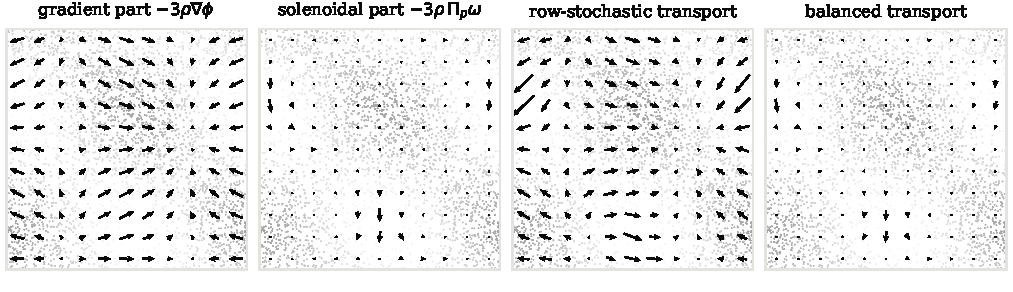
\includegraphics[width=\textwidth]{figures/torus_fields.pdf}
  \caption{Transport on the flat torus, drift $\omega=\rho(\nabla\phi+w)$
    with $\dv(p\,w)=0$, $\rho=0.3$, linear Randers cost, global bandwidth
    ($n=3000$, $h=0.04$). Arrows are averages over grid cells, all panels on
    one scale; grey dots are the samples, darker where $p$ is higher. The
    row-stochastic chain moves along the whole drift. The balanced chain
    moves along its $p$-solenoidal part only, as predicted by
    \cref{cor:laplace}.}
  \label{fig:fields}
\end{figure*}

\begin{table}[t]
  \caption{Bandwidth sweep at a fixed number of neighbours per kernel, $\rho=0.3$:
    slope of measured on predicted transport (1 is exact), and the
    gradient leak under per-row bandwidths with the cosine of its
    \cref{cor:leak} prediction.}
  \label{tab:sweep}
  \centering\small
  \begin{tabular}{@{}rrccc@{}}
    \toprule
    $h$ & $n$ & slope, Sk & slope, RS & per-row cos \\
    \midrule
    $0.070$ & $980$  & $0.69$ & $0.64$ & $0.95$ \\
    $0.050$ & $1920$ & $0.80$ & $0.78$ & $0.96$ \\
    $0.040$ & $3000$ & $0.84$ & $0.86$ & $0.96$ \\
    $0.035$ & $3918$ & $0.86$ & $0.89$ & $0.97$ \\
    \bottomrule
  \end{tabular}
\end{table}

\paragraph{Leakage.}
\Cref{fig:leak} compares a gradient drift with a solenoidal drift of the
same strength, under the three costs.
\begin{itemize}
  \item \textbf{Linear cost, global bandwidth.} The gradient drift
    produces no balanced transport, below $4\times10^{-11}$ for every
    $\rho$, at the level of the Sinkhorn tolerance
    (\cref{cor:gauge,cor:laplace}).
  \item \textbf{Linear cost, per-row bandwidth.} The gradient drift leaks
    at first order in $\rho$, and strongly: about $80\%$ of the transport
    produced by a solenoidal drift of the same strength. The leak matches
    \cref{cor:leak}(2) with cosine $0.96$ to $0.97$ and slope $0.92$. We
    obtain it from the measured per-row bandwidths through a weighted
    Helmholtz solve.
  \item \textbf{Squared cost, global bandwidth.} The leak is also linear in
    $\rho$ over the range we can simulate, at about $14\%$ of the
    transport of a solenoidal drift under the same cost. It shrinks when the sample size grows at fixed
    bandwidth ($0.020$, $0.017$, $0.013$ at $\rho=0.4$ for
    $n=980,1960,3920$, $h=0.07$), so it is at least partly a finite-sample
    effect. We do not reach the third-order regime of \cref{cor:leak}(1),
    and we leave its numerical confirmation open.
\end{itemize}

\begin{figure}[t]
  \centering
  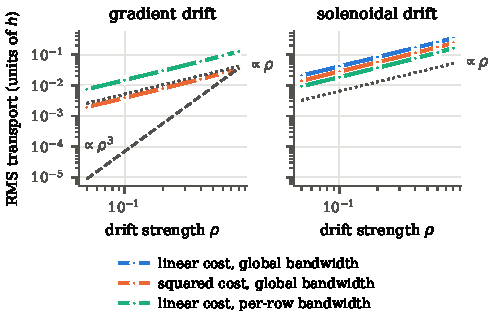
\includegraphics[width=\columnwidth]{figures/leakage.pdf}
  \caption{RMS balanced transport against drift strength on the torus
    ($n=3000$, $h=0.04$). Left: a gradient drift. With the linear cost and
    a global bandwidth it stays below $4\times10^{-11}$ for every $\rho$,
    outside the plotted range. Right: a solenoidal drift of the same
    strength, for reference.}
  \label{fig:leak}
\end{figure}


% ======================================================================
\section{Consequences for real velocity data}
\label{sec:real}

The theory predicts when a balanced affinity helps. What matters is how a
velocity field splits into a gradient part and a circulating part. We
decompose the edge flow $f_{ij}=\tfrac12(v_i+v_j)^\top(x_j-x_i)$ on a
30-nearest-neighbour graph in 30 principal components, following
\citet{jiang2011statistical}. The null model permutes the centred
velocities among cells.

\begin{table}[t]
  \caption{Hodge content of real RNA-velocity fields: share of
    $\|f\|^2$ carried by the gradient part, its permutation null, and the
    part that carries the ground-truth progress. Gastrulation:
    $n=30{,}000$ cells, E6.5--E8.5 \citep{pijuansala2019single}. RPE1:
    $n=2{,}793$ cells with FUCCI phase \citep{battich2020sequencing}, velocity
    from dynamo \citep{qiu2022mapping}.}
  \label{tab:hodge}
  \centering\small
  \begin{tabular}{@{}lccl@{}}
    \toprule
    velocity & gradient & null & progress carried by \\
    \midrule
    gastrulation, direct     & 0.93 & 0.33 & gradient \\
    gastrulation, scVelo     & 0.78 & 0.31 & gradient \\
    RPE1, direct             & 0.67 & 0.21 & non-gradient \\
    RPE1, dynamo kernel      & 0.29 & 0.24 & mostly non-gradient \\
    \bottomrule
  \end{tabular}
\end{table}

\Cref{tab:hodge} shows two opposite regimes.
\begin{itemize}
  \item \textbf{Developmental trajectories are gradient-dominated.} On
    gastrulation, a walk along the gradient part alone recovers the whole
    forward-in-time signal. The remainder carries none of it. A large share
    of the velocity is also a vector common to all cells, which
    \cref{cor:gauge} makes invisible to any balanced affinity.
  \item \textbf{The cell cycle circulates.} On RPE1, the gradient part of
    the direct velocity makes walks go slightly \emph{backwards} in phase.
    The non-gradient part carries the progress around the cycle; for the
    kernel velocity it carries most of it over long walks. The
    velocity circulates around closed loops through the phase bins far
    above the null ($z$ between $5$ and $18$).
\end{itemize}

\paragraph{Balanced versus row-stochastic affinities.}
\Cref{tab:dsrs} builds both affinities from the same velocity, with the
per-row perplexity calibration of practical neighbour embeddings.
\begin{table}[t]
  \caption{Balanced (Sk) versus row-stochastic (RS) Randers affinities
    built from the same velocity: squared cost, per-row perplexity
    $\sqrt n$, dense. ``cos'' is the mean cosine between each cell's shift
    in outgoing displacement, relative to the symmetric affinity, and the
    gradient or non-gradient Hodge part of the velocity. ``progress'' is
    the ground-truth progress after $10$ steps of the walk, minus that of
    the symmetric walk: pseudotime units for pancreas, fractions of a cycle
    for RPE1. The linear cost gives the same picture.}
  \label{tab:dsrs}
  \centering\small
  \begin{tabular}{@{}llrrr@{}}
    \toprule
    data & norm. & cos grad. & cos rest & progress \\
    \midrule
    pancreas      & RS & $0.56$ & $0.21$ & $0.167$ \\
                  & Sk & $0.38$ & $0.26$ & $0.000$ \\
    \addlinespace
    RPE1, direct  & RS & $0.56$ & $0.14$ & $0.060$ \\
                  & Sk & $0.01$ & $0.33$ & $0.082$ \\
    \addlinespace
    RPE1, kernel  & RS & $0.34$ & $0.36$ & $0.311$ \\
                  & Sk & $0.12$ & $0.37$ & $0.241$ \\
    \bottomrule
  \end{tabular}
\end{table}

Three observations follow the theory.
\begin{itemize}
  \item \textbf{No net progress along a potential.} On pancreas, the
    balanced walk's mean pseudotime gain is zero to numerical precision,
    as \cref{prop:netflow} requires. The row-stochastic walk gains steadily.
  \item \textbf{Circulation survives balancing.} On RPE1, the balanced walk
    keeps the progress around the cycle. With the direct velocity it
    progresses further than the row-stochastic walk, whose extra
    sensitivity to the gradient part pushes it backwards in phase.
  \item \textbf{The balanced shift drops the gradient part.} On RPE1 its
    correlation with the gradient part falls to about zero for the direct
    velocity, while its correlation with the remainder rises. On pancreas
    the balanced shift still has a sizeable gradient correlation. This is
    the first-order leak of per-row bandwidths (\cref{cor:leak}). By
    \cref{prop:netflow} it must be compensated, and it is: per pseudotime
    decile, the balanced chain moves cells forward in the first seven and
    backwards in the last three. Its largest step, $-0.076$, is in the
    terminal decile. The row-stochastic chain moves forward in every
    decile.
\end{itemize}


\paragraph{Consequence for embeddings.}
These numbers explain an observation from fitting Randers neighbour
embeddings on pancreas \citep{bastidasponce2019comprehensive}. With a
row-stochastic input affinity, the fitted flow agreed with the true
velocity at cosine $0.80$ and with scVelo's projection at $0.76$. With a
balanced one, these fell to $0.69$ and $0.54$. The balanced direction was
attenuated rather than erased, as \cref{cor:leak} predicts: per-row
bandwidths and the squared cost leak part of the gradient drift back.


% ======================================================================
\section{Related work}
\label{sec:related}

\paragraph{Entropic and balanced affinities.}
Perplexity-calibrated affinities come from SNE
\citep{hinton2002sne,vandermaaten2008tsne,vladymyrov2013entropic}. Doubly
stochastic normalisation was proposed for spectral clustering
\citep{zass2006doubly}. It has well-understood continuum limits for
symmetric kernels \citep{marshall2019manifold} and is robust to
heteroskedastic noise \citep{landa2021doubly}. SNEkhorn brought it to
neighbour embeddings with symmetry imposed \citep{vanassel2023snekhorn}.
All of these use symmetric costs or couplings; we balance an asymmetric
cost without imposing symmetry.

\paragraph{Directed kernels and their limits.}
\citet{perraultjoncas2011directed} split the continuum limit of a directed
kernel into a Laplacian and a drift. \citet{debaussart2026finslerian} build
Finsler kernels from directed distances and prove that the antisymmetric
part of the $\theta$-normalised operator converges to transport along the
centroid field. \Cref{thm:continuum} is the balanced counterpart, and it
shows that the choice of normalisation decides which Helmholtz component of
a drift is visible.

\paragraph{Hodge decompositions of flows.}
Combinatorial Hodge theory decomposes edge flows into gradient, curl and
harmonic parts \citep{jiang2011statistical,lim2020hodge}. Vector-field
reconstructions of single-cell dynamics analyse the same split
\citep{qiu2022mapping}. \citet{weinreb2018fundamental} show that snapshots
cannot identify the rotational part of a dynamics; \cref{sec:finite} shows
the complementary blindness of balanced affinities.

% ======================================================================
\section{Discussion and limitations}
\label{sec:discussion}

\paragraph{What changes in practice.}
For drifts dominated by their gradient part, such as developmental
trajectories, a balanced input affinity discards most of the direction,
while a row-stochastic one keeps it as a marginal tilt; an exact
potential cost then gives a reweighted symmetric affinity. For
circulating drifts, such as the cell cycle, balancing isolates the
circulation. Arrows drawn from a balanced embedding show a $p$-weighted
Helmholtz projection of the velocity, not the velocity itself.

\paragraph{Limitations.}
\Cref{thm:continuum} is formal: it rests on the small-noise ansatz for
Sinkhorn potentials, and a rigorous version would combine the consistency
arguments of \citet{debaussart2026finslerian} with quantitative stability
of Schr\"odinger potentials. It covers the first-order transport on a flat
torus with the frozen kernel, without curvature, boundaries or the
second-order Laplacian part. The third-order leak of the squared cost is
not observed numerically: at our sample sizes it leaks at first order,
with a constant that decreases with $n$. The \emph{output} kernel of an embedding, where
the same gauge acts on the fitted drift, is left to future work.

\bibliography{references}
\bibliographystyle{icml2026}

\newpage
\appendix
\onecolumn
\section{Computing Randers distances}
\label{app:randers}

\paragraph{Low dimension: eikonal solvers.}
For a fixed source $x_0$, $u=d_F(x_0\to\cdot)$ is the viscosity solution
of the eikonal equation $F^*_x(\nabla u)=1$, $u(x_0)=0$, where
$F^*_x(p)=\sup_{F_x(v)\le1}p^\top v$ is the dual norm. For a Randers norm
the dual is again of Randers type, given in closed form by Zermelo's
navigation \citep{bao2000introduction}. On a grid the equation is solved
by ordered-upwind methods \citep{sethian2003ordered} or by fast marching
with adaptive stencils, which handle anisotropic and asymmetric metrics
\citep{mirebeau2014efficient}. Each solve costs $O(N\log N)$ on $N$ grid
nodes, and the full cost matrix needs one solve per source, so $n$ solves.
This is practical in $d=2$ or $3$.

\paragraph{High dimension.}
A grid with $m$ nodes per axis has $m^d$ nodes, far out of reach for the
$10$ to $50$ principal components used on single-cell data. Graph
substitutes replace paths by chains of nearest-neighbour edges, each
carrying a local Randers length, and run Dijkstra's algorithm on the
directed graph, as Isomap does for Euclidean geodesics
\citep{tenenbaum2000global}. Heat-kernel proxies replace the infimum by a
small-time limit of a diffusion. Both converge only as the sampling
densifies around the optimal paths, which in high dimension takes
exponentially many points, and both are biased toward paths through
dense regions.

\paragraph{The drift is only sampled.}
A velocity is estimated at each point $x_i$ and nowhere else. The
infimum ranges over paths through regions where nothing is measured, so
the value of $d_F$ depends on how $\omega$ is extended between samples,
by interpolation or by a fitted network. That is a modelling choice the
data do not support.

\paragraph{Error of the closed forms.}
The straight segment $\gamma(t)=x_i+t\Delta$, $\Delta=x_j-x_i$, gives the
upper bound
\[
  d_F(x_i\to x_j)\le\|\Delta\|+\int_0^1\omega(x_i+t\Delta)^\top\Delta\,dt .
\]
Perturb the segment by $\eta(t)$ with $\eta(0)=\eta(1)=0$ and
$\|\eta\|\le h$. The length grows by order $h^2/r$, with $r=\|\Delta\|$.
The first variation of the drift term is
$\int_0^1\eta^\top(\nabla\omega-\nabla\omega^\top)\dot\gamma\,dt$, of
order $\|\nabla\omega-\nabla\omega^\top\|\,r\,h$; only the curl of
$\omega$ enters it. Optimising over $h$ gives a gain of order
$\|\nabla\omega-\nabla\omega^\top\|^2r^3$, which vanishes for gradient
drifts. The frozen form is the left-endpoint rule for the line integral,
with error $O(\|\nabla\omega\|r^2)$; the averaged form is the trapezoid
rule, with error $O(\|\nabla^2\omega\|r^3)$.

\section{Computations omitted from the main text}
\label{app:computations}

\paragraph{The Laplace--Randers partition function.}
For $\|\eta\|<1$ we claim $Z_d(\eta)=\int_{\R^d}e^{-\|v\|-\eta^\top v}dv=c_d\,(1-\|\eta\|^2)^{-(d+1)/2}$.
By rotation invariance $Z_d$ depends on $s=\|\eta\|$ only. In polar
coordinates, $Z_d(s)=\int_0^\infty r^{d-1}e^{-r}\,\Phi_d(sr)\,dr$, where
$\Phi_d(t)=\int_{S^{d-1}}e^{-t\theta_1}d\theta$. Three cases check the
claim directly:
\begin{itemize}
  \item $d=1$: $\int e^{-|v|-sv}dv=\frac{1}{1-s}+\frac{1}{1+s}=\frac{2}{1-s^2}$.
  \item $d=2$: $Z_2=2\pi\int_0^\infty re^{-r}I_0(sr)\,dr=2\pi(1-s^2)^{-3/2}$,
    the Laplace transform of $rI_0(sr)$ evaluated at $1$.
  \item $d=3$: $Z_3=\frac{4\pi}{s}\int_0^\infty re^{-r}\sinh(sr)\,dr=8\pi(1-s^2)^{-2}$.
\end{itemize}
For general $d$, $\Phi_d(t)=c'_d\,t^{-(d-2)/2}I_{(d-2)/2}(t)$, and the
Laplace transform of $r^{d/2}I_{(d-2)/2}(sr)$ at $1$ is proportional to
$s^{(d-2)/2}(1-s^2)^{-(d+1)/2}$. This gives the claim.
Differentiating \eqref{eq:laplace} in $\zeta$ gives
$M(\omega,\zeta)=-(d+1)\,\eta/(1-\|\eta\|^2)$ with $\eta=\omega-\zeta$.

\paragraph{The Randers unit ball.}
$\{v:\|v\|+\omega^\top v\le1\}$ is the set where $\|v\|^2\le(1-\omega^\top v)^2$
and $\omega^\top v\le1$. For $\|\omega\|<1$ this is an ellipsoid, symmetric
about the axis $\omega$. Along that axis, $v=t\,\omega/\|\omega\|$ with
$t\in[-1/(1-\|\omega\|),\,1/(1+\|\omega\|)]$. Its centre is therefore
$c_F=-\omega/(1-\|\omega\|^2)$. With $\kappa_g=d+1$ for $g=e^{-t}$, this
agrees with $M(\omega,0)$ above.

\paragraph{Linearisation for the Gaussian profile.}
For $g(t)=e^{-t^2/2}$,
$F_\omega(v)^2=\|v\|^2+2\|v\|\,\omega^\top v+(\omega^\top v)^2$. To first
order in $(\omega,\zeta)$ the tilted density is
$\mathcal{N}(0,I_d)\cdot\big(1+\zeta^\top v-2\|v\|\,\omega^\top v\big)$.
Its mean is
\[
  \zeta-2\,\E\big[\|v\|\,vv^\top\big]\,\omega=\zeta-\frac{2\,\E\|v\|^3}{d}\,\omega .
\]
So $s_0=2\E\|v\|^3/d$; in $d=2$, $\E\|v\|^3=3\sqrt{\pi/2}$ and
$s_0\approx3.76$. The map $(\omega,\zeta)\mapsto M$ is odd, so the next
term is cubic.

\paragraph{Per-row bandwidths in the discrete prediction.}
\Cref{sec:exp} compares measured transport with \cref{cor:leak}(2). It uses
the discrete form of that statement. With kernel $\exp(-\beta_iC_{ij})$ and
$\beta(x)=1/(h\sigma(x))$, the predicted mean displacement is
$-(d+1)\,u/\beta^2$. Here $u=\beta\omega-\nabla\Psi$ is the solenoidal
part of $\beta\omega$ in $L^2(p/\beta^2)$. We compute it by finite volumes
on a $128\times128$ periodic grid, after smoothing $1/\beta_i$ onto the
grid with a Gaussian of width $0.04$.

\section{Experimental protocol}
\label{app:protocol}

All experiments run in float64 with log-domain Sinkhorn, stopped when every
row sum is within $10^{-11}$ relative error. Code:
\texttt{experiments/theory/gauge\_checks.py}.

\paragraph{Finite-sample identities.}
$n=400$ Gaussian points in $\R^5$, $\eps=0.3$, Euclidean $S$. The gradient
part uses $\phi=0.2(\tanh x_1+0.3x_2^2)$; the generic antisymmetric part is
a random Gaussian matrix, antisymmetrised, of scale $0.1$.

\paragraph{Torus.}
Points are sampled on $\T^2$ by rejection from
$p(x)\propto1+0.6\cos(2\pi x_1)\cos(2\pi(x_2-0.15))+0.25\sin(2\pi(x_1+x_2))$.
\begin{itemize}
  \item Gradient part: $\phi=\big(\sin 2\pi x_1+\tfrac12\sin 2\pi(x_2+0.2)\big)/2\pi$.
  \item Solenoidal part: $w=p^{-1}\nabla^\perp\chi$ with
    $\chi=\sin(2\pi x_1)\sin(2\pi x_2)/2\pi$, so that $\dv(p\,w)=0$ by
    construction. Hence $\Leray_p(\nabla\phi+w)=w$ exactly.
\end{itemize}
Both fields are scaled to maximum norm $1$ and multiplied by $\rho$. The
cost is the linear Randers cost with the exact potential term and the
averaged form for $w$:
$C_{ij}=\|\Delta_{ij}\|+\rho(\phi_j-\phi_i)+\rho\,\bar w_{ij}^\top\Delta_{ij}$,
with torus displacements. The transport field is
$b_i=h^{-1}\sum_jP_{ij}\Delta_{ij}/\sum_jP_{ij}$. The same quantity for
the drift-free kernel is subtracted, to remove the $O(h)$ density term.
Per-row bandwidths are calibrated by bisection to perplexity $30$.

\section{Proof sketch of \cref{thm:continuum}}
\label{app:continuum}

\begin{proof}[Proof sketch of \cref{thm:continuum}]
  \emph{Step 1: local profile.} Substitute $y=x+h\sigma(x)v$. Then
  $v_h(y)/v_h(x)=\exp\!\big(\sigma\nabla\Psi(x)^\top v+O(h\|v\|^2+h\|v\|)\big)$
  and $p(y)/p(x)=1+O(h\|v\|)$. So the law of $v$ under $T_h(x,\cdot)$
  converges to the normalised density
  $g(F_{\omega(x)}(v))\,e^{\sigma\nabla\Psi^\top v}$. Its mean is
  $M(\omega,\sigma\nabla\Psi)$, and the displacement is $h\sigma v$, which
  gives \eqref{eq:b}. Tails are controlled because the tilt stays inside
  the domain of $\Lambda$.

  \emph{Step 2: stationarity.} For $f\in C^2$, stationarity of $p$ gives
  $\int p(x)\int\big(f(y)-f(x)\big)T_h(x,dy)\,dx=0$. A Taylor expansion
  turns this into $h\int p\,b_h^\top\nabla f+O(h^2)=0$. Hence
  $\int p\,b^\top\nabla f=0$ for all $f$, i.e.\ $\dv(p\,b)=0$.

  \emph{Step 3: variational form.} The first variation of \eqref{eq:J} is
  $\delta J=\int p\,\sigma\,\nabla_\zeta\Lambda^\top\nabla\delta\Psi
  =-\int\dv(p\,b)\,\delta\Psi$. So Step 2 is the Euler--Lagrange equation
  of $J$. Strict convexity of $\Lambda$ in $\zeta$ makes the critical
  point unique up to constants.

  \emph{Row-stochastic case.} There is no tilt, so the mean is $M(\omega,0)$.
  Write $g(F)=\int_0^\infty|g'(t)|\,\1\{F\le t\}\,dt$ and use the
  1-homogeneity of $F$: $\int v\,\1\{F(v)\le t\}\,dv=t^{d+1}\!\int_{\{F\le1\}}v\,dv$.
  The ratio of the first moment to the mass gives $\kappa_g c_F$.
\end{proof}

\begin{proof}[Proof of \cref{cor:laplace}]
  (1) The integrand $-\log(1-t^2)$ is non-negative and vanishes only at
  $t=0$. If $\omega=\nabla\phi$, then $\Psi=\phi$ attains the minimum
  value $0$ and $b=0$. Conversely, $b=0$ forces $\omega=\nabla\Psi$.
  (2) Since $-\log(1-t^2)=t^2+O(t^4)$, $\Psi$ minimises
  $\int p\,\|\omega-\nabla\Psi\|^2$ to leading order, which is the weighted
  $L^2$ projection onto gradients.
\end{proof}


\end{document}
